\documentclass[a4paper]{article}

\usepackage{array}
\usepackage{longtable}
\usepackage{graphicx}
\usepackage[a4paper, body={17cm, 26cm}]{geometry}
\usepackage{listings}


\begin{document}
\lstset{language=C++, basicstyle=\small, showstringspaces=false}

\begin{center}
\textbf{\LARGE Guidelines for using the library}
\end{center}

\vspace{1cm}
\noindent In this document you will find the guidelines for using the library on a Linux system.

%***************************************************************************************************************************************
%
% Section
%
%***************************************************************************************************************************************

\section{Console execution}

Access to the directory cgal and do the following:

\begin{verbatim}
$ make
$ ./boolop file_subject file_clipping
\end{verbatim}

\noindent where:

\begin{itemize}
 \item \verb+file_subject+ is the file containing the subject polygon
 \item \verb+file_clipping+ is the file containing the clipping polygon
 \item \verb+file_result+ will be used to save the result of the operation
 \item the last parameter is optional and indicates the kind of Boolean operation:
   \begin{itemize}
    \item I stands for Intersection (the default operation)
    \item U stands for Union
    \item D stands for Difference between the subject and clipping polygons
    \item X stands for eXclusive OR (Symmetric difference) between the subject and clipping polygons
   \end{itemize}
\end{itemize}

The implementation is based on CGAL, so you need this library for a correct compilation. In the directory \textit{cpp} you can find a
non-robust implementation of the algorithm using only C++ code.

%***************************************************************************************************************************************
%
% Section
%
%***************************************************************************************************************************************

\section{Format of polygon files}
You can find polygons in the directory \textit{polygons}. In the directory \textit{polygons/random} you will find random non-self-intersecting polygons 
up to 10000 vertices. You can, for example, try:

\begin{verbatim}
$ ./boolop ../../polygons/random/p10000-0 ../../polygons/random/p1000-0
\end{verbatim}

You can also create your own polygons. A text file containing a polygon has the following structure:

\begin{verbatim}
<number of contours>
<number of vertices of first contour>
<vertex-list of first contour>
<number of vertices of second contour>
<vertex-list of second contour>
...
<contourId>: <firstHole_contourId> <secondHole_contourId> ...
...
\end{verbatim}

Next, you can see the content of the file \textit{polygonwithtwocontours}, that belongs to the directory \textit{polygons/samples}---see 
Figure \ref{twocontours}:

\begin{verbatim}
2
3
   0.1 0.1
   0.3 0.1
   0.2 0.3
3
   0.6 0.1
   0.8 0.1
   0.7 0.3
\end{verbatim}

%
% FIGURE: polygonwithtwocontours
%
\begin{figure}
\centering
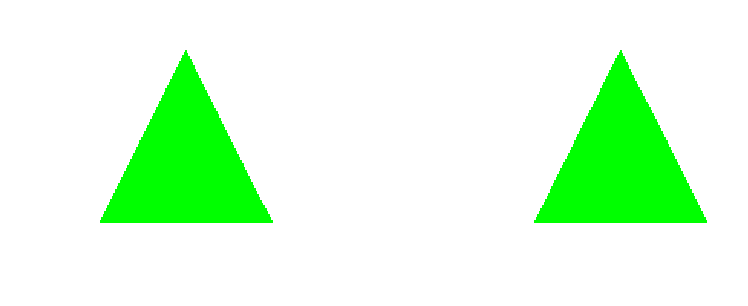
\includegraphics[scale=0.5]{twocontours.eps}
\caption{Polygon with two contours.}
\label{twocontours}
\end{figure}

As an example of a text file representing a polygon with holes you can see the file \textit{polygonwithholes}, that belongs to the 
directory \textit{polygons/samples}---see Figure \ref{holes}:

\begin{verbatim}
3
3
	-0.15 -0.15
	0.45 -0.15
	0.15 0.45
3
	-0.05 -0.05
	0.15 0.35
	0.35 -0.05
3
	0.05 0.05
	0.25 0.05
	0.15 0.25
0: 1
1: 2
\end{verbatim}

The line \verb+0: 1+ means that the first specified contour has a hole: the sencond specified contour. The line \verb+1: 2+ means that the 
second specified contour has a hole: the third specified contour. Contours's IDs start from 0.

The algorithm works fine with polygons which holes are not specified. Anyway, the algorithm computes holes information, and writes text files
representing polygons with holes information.

%
% FIGURE: polygonwithtwocontours
%
\begin{figure}
\centering
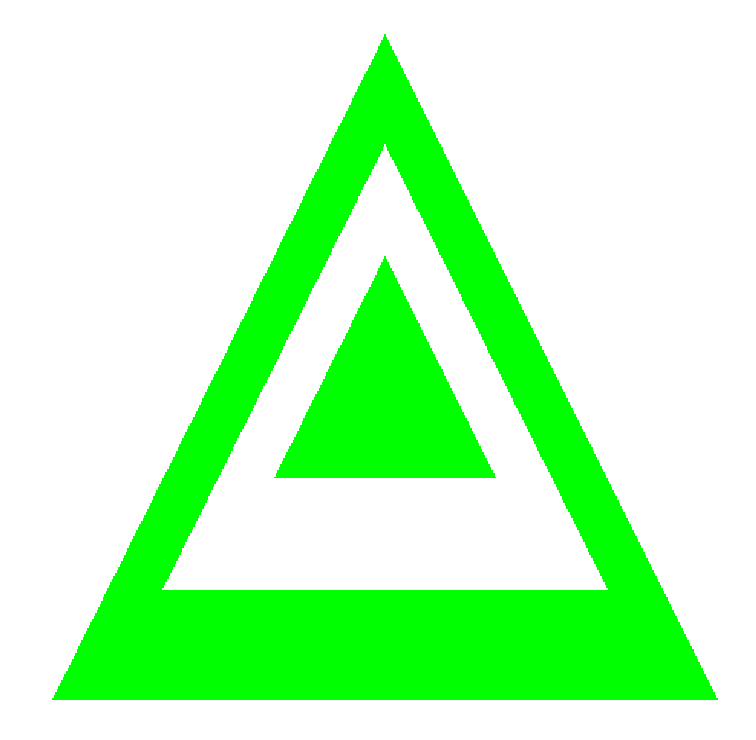
\includegraphics[scale=0.3]{holes.eps}
\caption{Polygon with holes.}
\label{holes}
\end{figure}

%***************************************************************************************************************************************
%
% Section
%
%***************************************************************************************************************************************

\section{Admitted input polygons}

The following features are allowed in input polygons:
\begin{itemize}
 \item Contours can be described in clockwise or counterclockwise order.
 \item Polygons can have holes. However, you do not need to specify what contour are holes.
 \item A vertex of a polygon can touch (in a point) a vertex or edge of the same polygon.
 \item Self-intersecting polygons.
\end{itemize}

The following features are not allowed in input polygons:
\begin{itemize}
 \item Overlapping edges (the intersection of two edges of the same polygon can be a point, but cannot be a segment).
\end{itemize}

The result polygon computed by the algorithm contains holes information. Furthermore, external contours are counterclockwise oriented. If a
result polygon contains holes then ``odd depth holes'' are clockwise oriented and ``even depth holes'' are counterclockwise oriented.


%***************************************************************************************************************************************
%
% Section
%
%***************************************************************************************************************************************

\section{Rendering the result of Boolean operations}

If you want to render the result of a Boolean operation you should have installed Qt and OpenGL and type:

\begin{verbatim}
$ cd qt
$ qmake qt.pro
$ make
$ ./qt
\end{verbatim}

This program includes an interesting option to watch step by step the computation of the Boolean operation.

%***************************************************************************************************************************************
%
% Section
%
%***************************************************************************************************************************************

\section{License Issues}

If you want to use the CGAL based implementation you must consult the CGAL's license policy. The C++ implementation is public domain software. For
the code based on Qt you must consult the Qt's license policy.

%***************************************************************************************************************************************
%
% Section
%
%***************************************************************************************************************************************

\section{Performance and robustness}

The code based on CGAL uses an exact kernel, so it should be robust. The code based on C++ is not robust, however is quite faster than the
code based on CGAL.

%%%%%%%%%%%%%%%%%%%%%%%%%%%%%%%%%%%%%%%%%%%%%%%%%%%%%%%%%%%%%%%%%%%%%%%%%%%%%%%%%%%%%%%%%%%%%%%%%%%%%%%%%%%%%%%%%%%%%%%%%%%%%%%%%%%%%%%%%
% Section: Acknowledgements
%%%%%%%%%%%%%%%%%%%%%%%%%%%%%%%%%%%%%%%%%%%%%%%%%%%%%%%%%%%%%%%%%%%%%%%%%%%%%%%%%%%%%%%%%%%%%%%%%%%%%%%%%%%%%%%%%%%%%%%%%%%%%%%%%%%%%%%%%

\section{Acknowledgements}

I would like to thank Antonio J. Rueda for his ideas to the early versions of the code. I would also like to thank Christian Woltering for his corrections in the function \lstinline+Polygon::operator>>+ and for formulating a correct
definition of the field \lstinline+posSL+ of the \lstinline+SweeEvent+ structure.


\end{document}